\documentclass[tikz]{standalone}
\usepackage{tikz}

\usetikzlibrary{arrows.meta,bending,chains,decorations.markings}
\tikzset{% 
    attach arrow/.style={
    decoration={
        markings,
         mark=at position 0 with {\pgfextra{%
         \pgfmathsetmacro{\tmpArrowTime}{\pgfkeysvalueof{/tikz/arc arrow/length}/(\pgfdecoratedpathlength)}%
         \xdef\tmpArrowTime{\tmpArrowTime}}},
        mark=at position {#1-3*\tmpArrowTime} with {\coordinate(@1);},
        mark=at position {#1-2*\tmpArrowTime} with {\coordinate(@2);},
        mark=at position {#1-1*\tmpArrowTime} with {\coordinate(@3);},
        mark=at position {#1+\tmpArrowTime/2} with {\coordinate(@4);
        \draw[-{Stealth[length=\pgfkeysvalueof{/tikz/arc arrow/length},bend]}] plot[smooth]
         coordinates {(@1) (@2) (@3) (@4)};},
        },
     postaction=decorate,
     },
     attach arrow/.default=0.5,
     arc arrow/.cd,length/.initial=2mm,
}

\tikzstyle{conv} = [rectangle, draw=black, fill=blue]
\tikzstyle{pool} = [rectangle, draw=black, fill=red]
\tikzstyle{scat} = [rectangle, draw=black, fill=blue]
\tikzstyle{dense} = [rectangle, draw=black, fill=green]
\tikzstyle{arrow} = [thick, ->, >=stealth]

\begin{document}
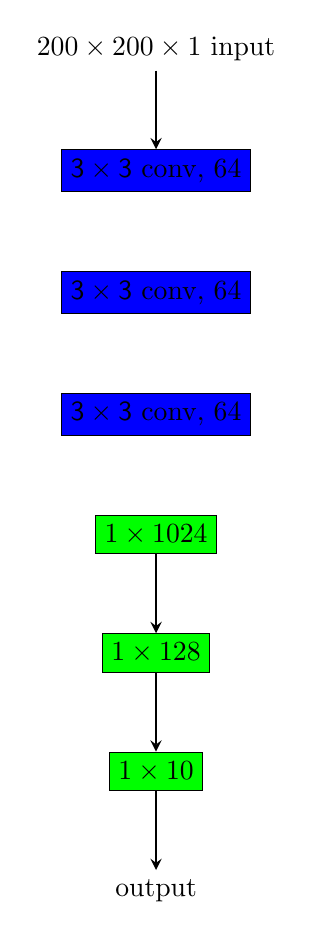
\begin{tikzpicture}
% [font=\sffamily,>={Stealth[bend]},
%     block/.style={draw, rectangle,minimum height=1.6em,minimum width=9em,
%     rotate=90,},decide/.code={\ifnum#1<7
%      \tikzset{fill=purple!10,execute at begin node={$\mathsf{3}\times\mathsf{3}$ conv, 64}}
%     \else
%      \tikzset{fill=green!10,execute at begin node={$\mathsf{3}\times\mathsf{3}$ conv, 128}}
%     \fi}]
%  \begin{scope}[start chain=A placed {at={(\tikzchaincount*3em,0)}},
%     nodes={on chain,block,join= by {thick,->},decide=\tikzchaincount}]
%     \path foreach \X in {1,...,6}{node{}}
%       node{/2}
%       foreach \X in {1,...,7}{node{}};
%  \end{scope}


    \node (in0) {$200 \times 200 \times 1$ input};

    \node (conv0) [conv, below=of in0] {$\mathsf{3}\times\mathsf{3}$ conv, 64};
    \node (pool0) [conv, below=of conv0] {$\mathsf{3}\times\mathsf{3}$ conv, 64};
    \node (conv1) [conv, below=of conv0] {$\mathsf{3}\times\mathsf{3}$ conv, 64};
    \node (conv2) [conv, below=of conv1] {$\mathsf{3}\times\mathsf{3}$ conv, 64};
    \node (lin0) [dense, below=of conv2] {$1 \times 1024$};
    \node (lin1) [dense, below=of lin0] {$1 \times 128$};
    \node (lin2) [dense, below=of lin1] {$1 \times 10$};

    \node (out0) [below=of lin2] {output};

    \draw [arrow] (in0) -- (conv0);
    \draw [arrow] (lin0) -- (lin1);
    \draw [arrow] (lin1) -- (lin2);
    \draw [arrow] (lin2) -- (out0);

%  \foreach \X in {1,...,7}
%  {\draw[thick,attach arrow] \ifnum\X=4 [dashed]\fi 
%  (-4.5em+\X*6em,0) to[out=90,in=180] 
%  (-1.5em+\X*6em,7em) to[out=0,in=90] (1.5em+\X*6em,0);
%  }
%  \path (A-1.north) -- ++ (-2em,0) node[anchor=south,rotate=90](pool){pool}
%   -- ++ (-4em,0) node[block,anchor=south,fill=orange!10](A-0)
%      {$\mathsf{3}\times\mathsf{3}$ conv, 64};
%  \draw[thick,->] (A-0) -- (pool);
%  \draw[thick,->] (pool) -- (A-1);
%  \draw[thick,<-] (A-0) -- ++ (-6em,0);
\end{tikzpicture}


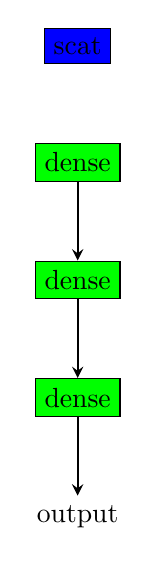
\begin{tikzpicture}
    \node (scat) [scat] {scat};
    \node (lin0) [dense, below=of scat] {dense};
    \node (lin1) [dense, below=of lin0] {dense};
    \node (lin2) [dense, below=of lin1] {dense};
    \node (out0) [below=of lin2] {output};

    \draw [arrow] (lin0) -- (lin1);
    \draw [arrow] (lin1) -- (lin2);
    \draw [arrow] (lin2) -- (out0);
\end{tikzpicture}

\end{document}